
\subsection{Multi-Zonal Specialization: Routing Tasks Across Heterogeneous Substrates}
\label{subsec:multizonal}

\marginpar{Zones = different physics, different priors.}
Beyond segmentation, animals exhibit \emph{multi-zonal specialization}: regions (neural and non-neural) with distinct morphologies, materials, timescales, and couplings.
In the SMN, zones constitute \emph{heterogeneous control substrates}---some excitable and fast, others viscoelastic and slow; some tightly gap-junction coupled, others diffusively or mechanically coupled.
Zonation enables \emph{routing}: \NAP{}s flexibly recruit different zones as the situation demands, while \TAP{}s arise only when negotiable patterns leave \emph{public traces} (marks, deposits, shared states) that become accessible to other agents.

\paragraph{Evo--devo foundations: regionalization across taxa.}
Regional identities arise by conserved patterning programs that parcel the organism into \emph{fields} with distinct control opportunities.
Hindbrain rhombomeres provide a canonical example of serial regionalization with sharp lineage boundaries and specific projections \cite{LumsdenKrumlauf1996Hindbrain}.
Forebrain arealization follows the prosomeric model of nested longitudinal and transverse domains \cite{PuellesRubenstein2003Prosomeric}.
At the cortical level, early patterning sets up area biases that later experience can refine \cite{SurRubenstein2005CortexPatternPlasticity}.
Outside the CNS, arthropod \emph{tagmosis} (head, thorax, abdomen) illustrates regional specialization of repeated elements into functionally distinct zones \cite{Scholtz2010Tagmosis}.

\paragraph{Zonation as control architecture.}
Zones differ in transfer functions and priors: elastic vs rigid, high- vs low-pass, excitable vs passive.
The SMN exploits these differences by \emph{task matching}: predictive smoothing in viscoelastic zones; precise timing in excitable zones; persistent bias in bioelectricly polarized zones \cite{Levin2014MolecularBioelectricity}.
Cerebellar microzones and their olivo-cerebellar loops exemplify fine-grained error-driven control layered on top of slower postural zones \cite{AppsHawkes2009CerebellarZones}; basal ganglia–thalamocortical loops instantiate selection/routing among competing controllers \cite{AlexanderDeLongStrick1986ParallelLoops}.
\NAP{}s provide the negotiable substrate that allows such heterogeneous zones to be flexibly recombined.

\paragraph{Habitat coupling.}
Zones are differentially exposed to the medium: distal appendage zones interact with boundary layers and wakes; axial postural zones bear gravitational loading; epithelial exchange zones sense and shape flow/chemistry.
The habitat thus supplies \emph{zone-specific statistics} that the SMN learns to rely on for \NAP{} routing.
When such patterns are externalized into stable environmental modifications, they become \TAP{}s---for example, building nests, laying chemical trails, or leaving marks that other agents can read.

\paragraph{Thermodynamic economy.}
Specialization reduces internal erasures: rather than rewriting a monolithic controller, the SMN composes \NAP{}s by switching among zones with \emph{pre-tuned priors}, minimizing logically irreversible policy overwrites \cite{Landauer1961Irreversibility,Bennett2003LandauerNotes}.
Where durable public traces are beneficial, \TAP{}s exploit stable substrates (mud, fiber, pheromonal fields), offloading memory to the habitat and anchoring intersubjective coordination.
\paragraph{Formalization sketch.}
Let $x_i(t)$ be the state of the $i$th segmental controller (e.g., a central pattern generator modeled as a phase oscillator).
Nearest-neighbor coupling $K_{ij}$ yields traveling waves or standing patterns depending on phase-lag targets.
In the simplest case, a lattice of oscillators (Kuramoto-type) produces smooth waves; \emph{interrupts} are transient detunings or phase resets at select nodes.
\begin{align}
\dot{\theta}_i &= \omega_i + \sum_{j \in \mathcal{N}(i)} K_{ij} \sin(\theta_j - \theta_i - \phi_{ij}) + u_i(t),
\end{align}
where $u_i(t)$ captures modulatory inputs from the SMN:
\begin{itemize}
  \item \textbf{FAPs} are stereotyped oscillatory routines (the baseline $\omega_i$ dynamics).
  \item \textbf{HAPs} introduce haltability: $u_i(t)$ imposes temporary pauses or resets.
  \item \textbf{NAPs} implement negotiable coordination: rephasing or reweighting of couplings $K_{ij}$ under perceptual predicates (affordance tests).
  \item \textbf{TAPs} arise only when such negotiable patterns leave external traces (gesture, vocalization, artifact), becoming available for intersubjective transaction.
\end{itemize}
\marginpar{Kuramoto lattice as a \emph{control surface}.}
\todo{Figure: (i) segmented chain with CPGs, (ii) phase-lag targets for swimming/walking, (iii) local phase reset producing a step or turn, (iv) habitat arrows (gravity/fluid) shaping feasible lags.}

\begin{figure}[ht] 
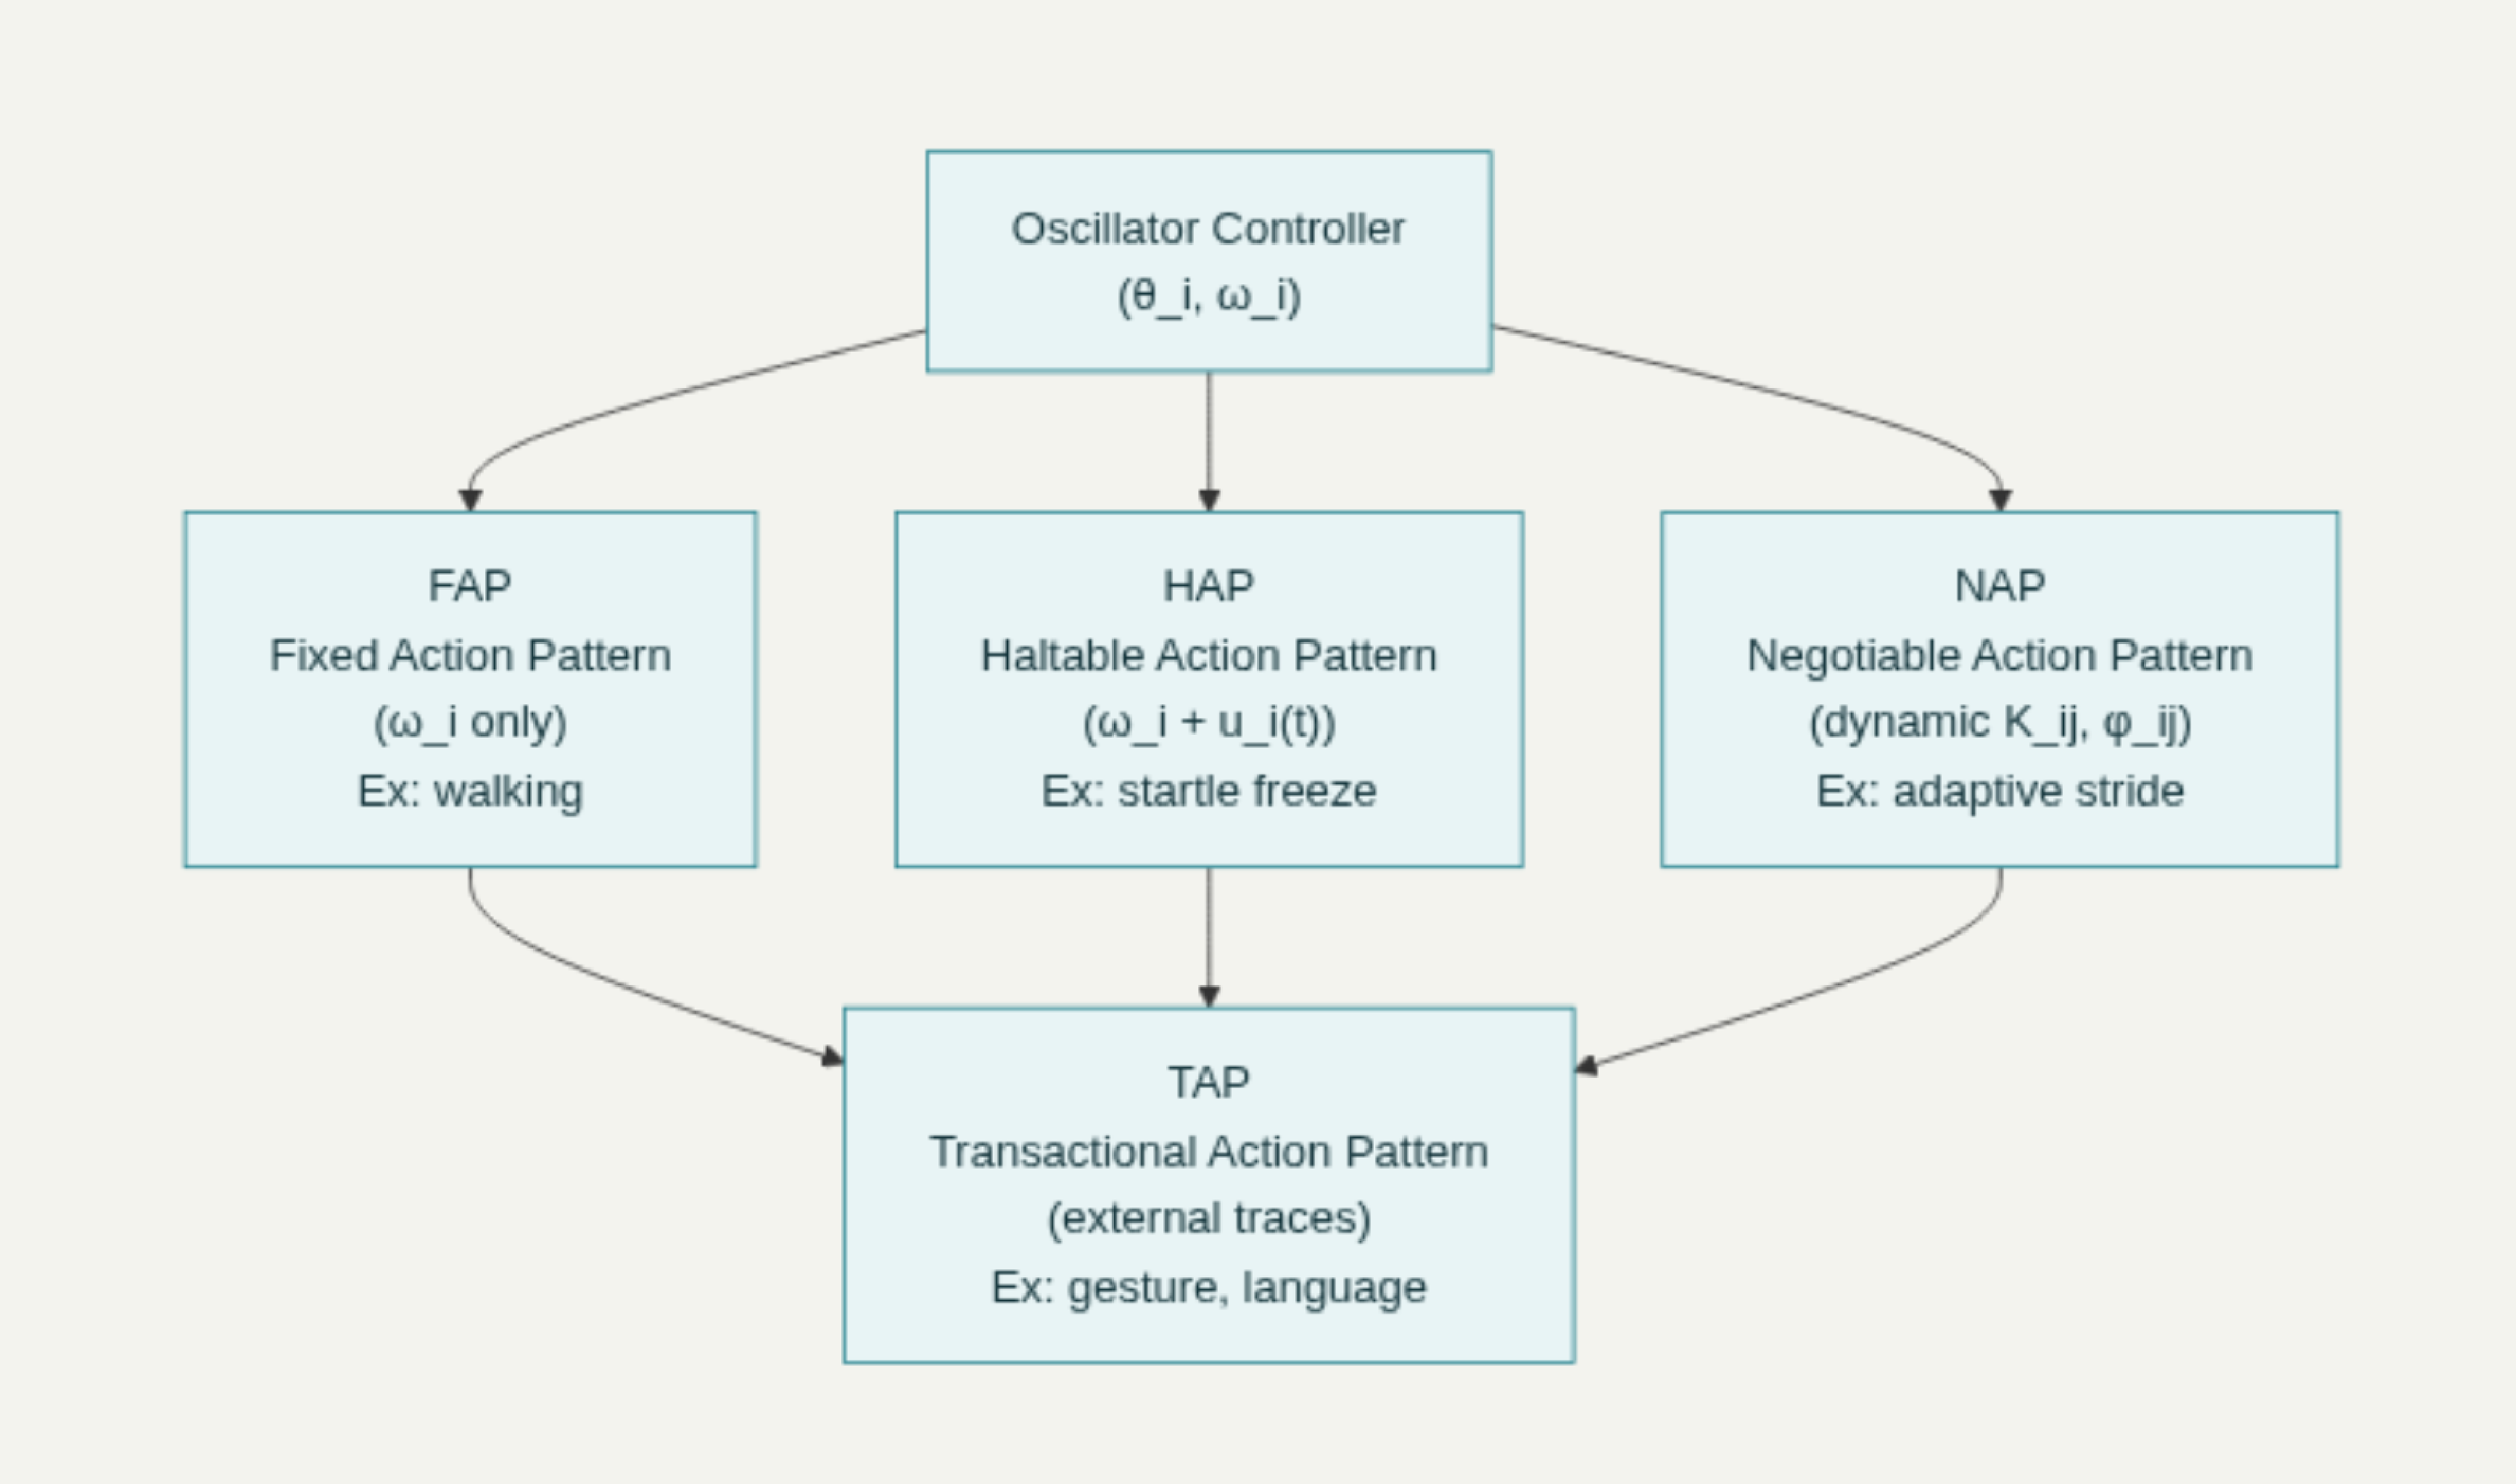
\includegraphics[width=\textwidth]{graphics/FAP-HAP-NAP-TAP-2.pdf}
\caption{A diagram that visually organizes the relationships between FAP, HAP, NAP, and TAP, showing how each category connects to oscillator-based control terms and behavioral examples. The flowchart starts from the oscillator-based controller, branches to FAP, HAP, and NAP, and then leads from NAP to TAP, illustrating the hierarchical structure and characteristic mechanisms for each pattern type. For example, walking corresponds to FAP, startle freeze to HAP, adaptive stride to NAP, and their traces accessible external to thhe agent become potential TAP. Each node is annotated with both the formal control expression and a real-world illustration, clarifying the progression from innate rhythms to socially communicable actions.}\label{schematic-fhnt-ap}
\end{figure}

\paragraph{SMN vs Habitat (capsule).}
\textbf{SMN:} segmental CPGs coordinate via local phase rules; interrupts compose into \NAP{}s, which provide the substrate for adaptive negotiation.  
\textbf{Habitat:} environmental structure (e.g., gravity, buoyancy, fluid drag) shapes feasible phase-lags, constraining and simplifying coordination.  

\paragraph{Adaptation.}
Segmental CPGs adapt phase and gain through local plasticity while surrounding tissues update bioelectric set-points, stabilizing useful NAPs (e.g., common gaits) and enabling rapid local interrupts without global rewrites.  
Segmentation thus discretizes control into re-usable modules: \emph{FAPs become haltable, HAPs become negotiable, and NAPs can be externalized as TAPs}.  
The SMN leverages these synergies to retime and recombine actions with low wiring cost \citep{BizziCheung2013}.


